\documentclass{standalone}
\usepackage{tikz}
\usetikzlibrary{patterns, positioning}
\usepackage[sfdefault]{ClearSans} %% option 'sfdefault' activates Clear Sans as the default text font
\usepackage[T1]{fontenc}

\begin{document}
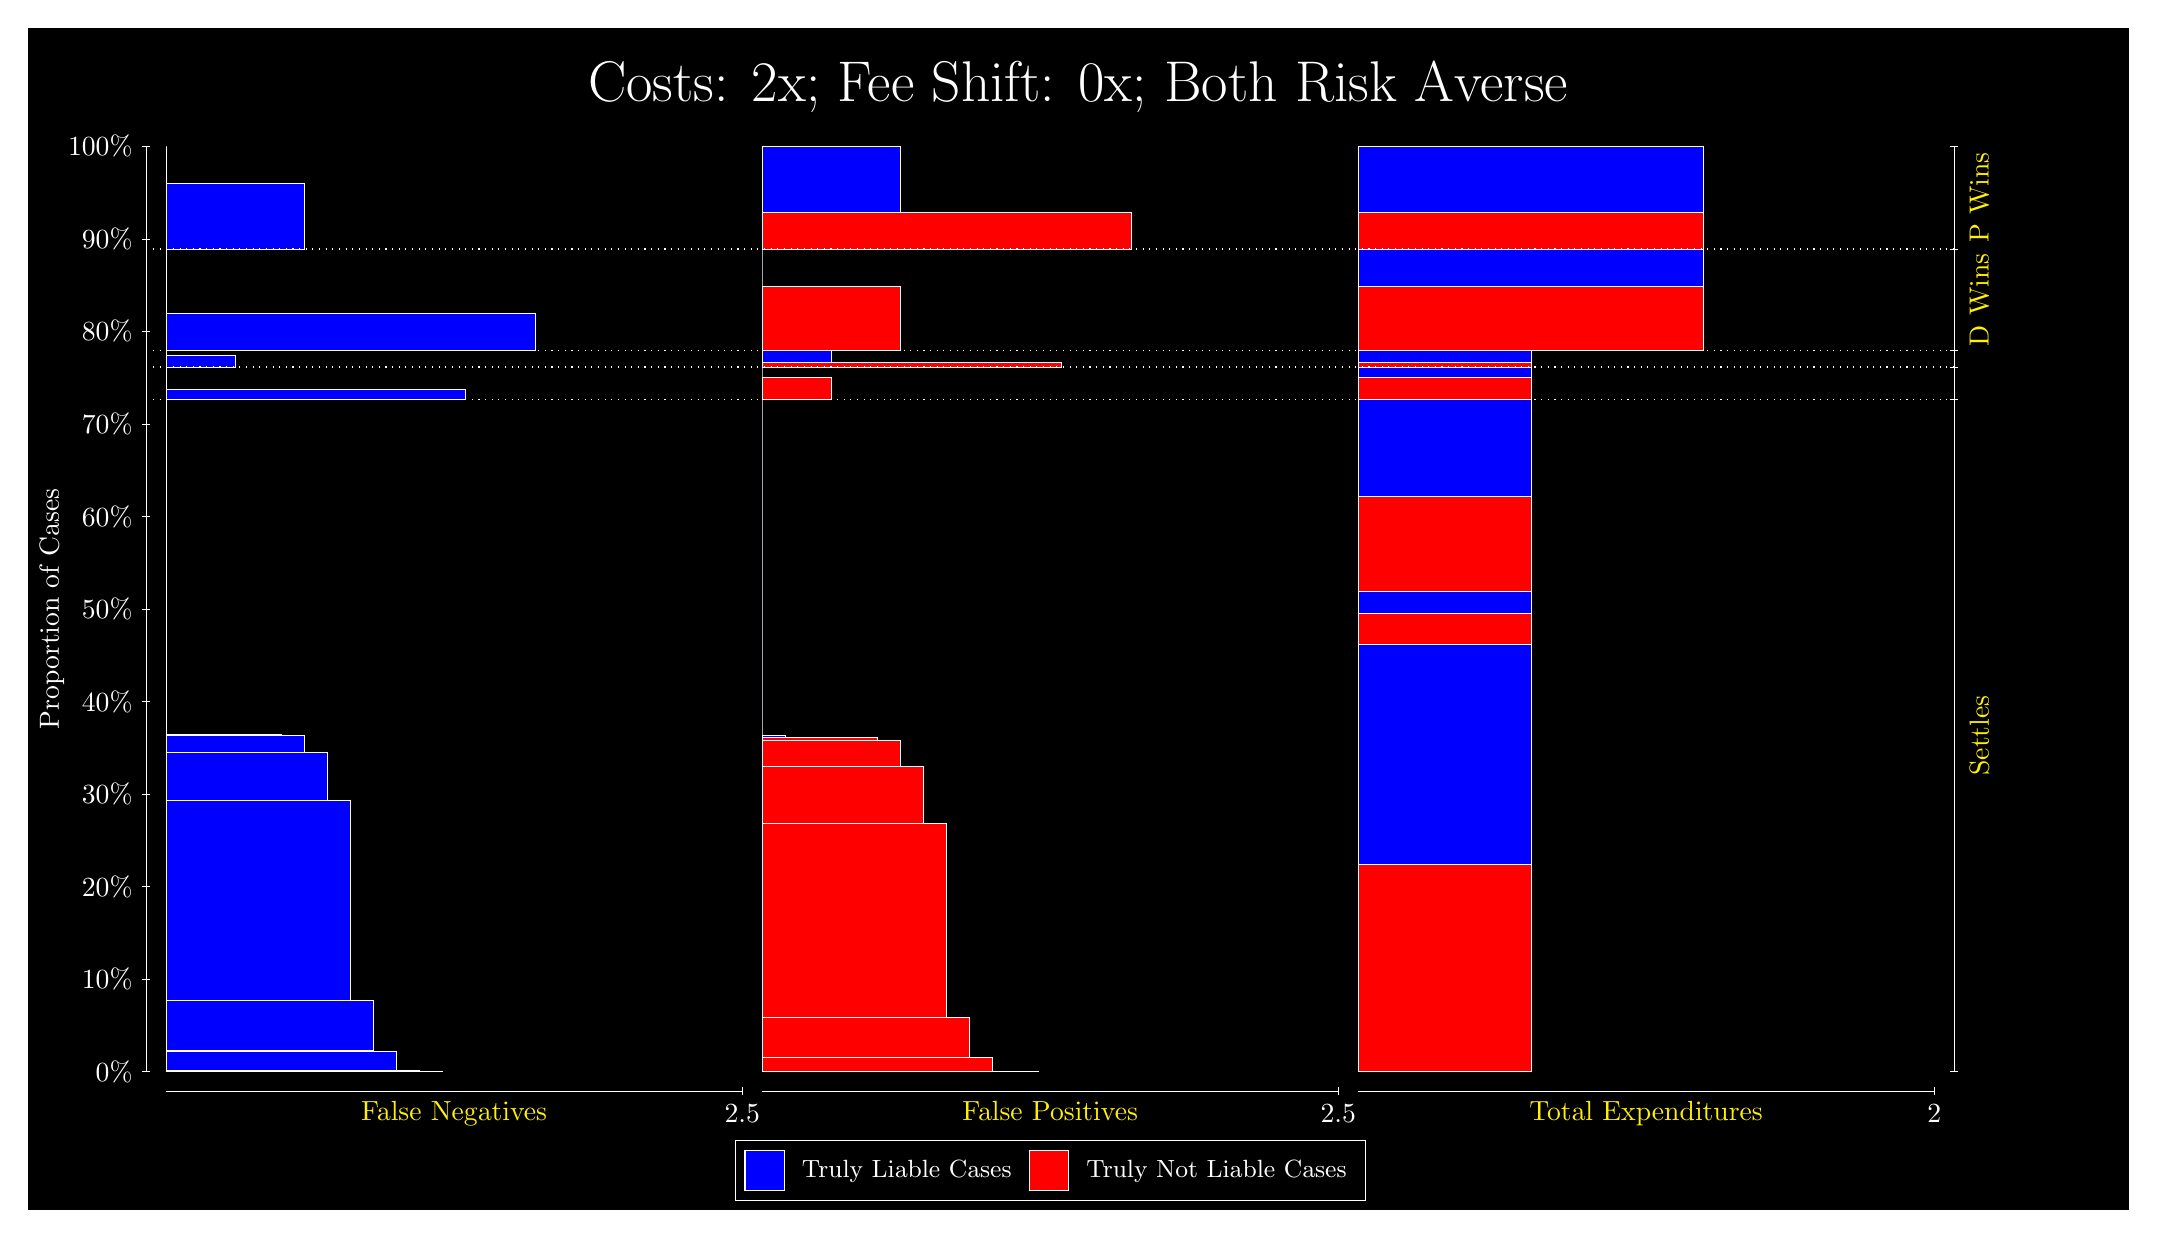
\begin{tikzpicture}
\draw[fill=black] (0,0) rectangle (26.667,15);
\draw[text=white] (0,13.5) rectangle (26.667,15) node[midway] {\huge Costs: 2x; Fee Shift: 0x; Both Risk Averse};
\draw[white, very thin] (1.5,1.75) -- (1.5,13.5);
\node[rotate=90, text=white, anchor=center] at (0.3, 7.625) {Proportion of Cases};
\draw[white, very thin] (1.45,1.75) -- (1.55,1.75);
\node[text=white, anchor=east] at (1.45, 1.75) {0\%};
\draw[white, very thin] (1.45,2.925) -- (1.55,2.925);
\node[text=white, anchor=east] at (1.45, 2.925) {10\%};
\draw[white, very thin] (1.45,4.1) -- (1.55,4.1);
\node[text=white, anchor=east] at (1.45, 4.1) {20\%};
\draw[white, very thin] (1.45,5.275) -- (1.55,5.275);
\node[text=white, anchor=east] at (1.45, 5.275) {30\%};
\draw[white, very thin] (1.45,6.45) -- (1.55,6.45);
\node[text=white, anchor=east] at (1.45, 6.45) {40\%};
\draw[white, very thin] (1.45,7.625) -- (1.55,7.625);
\node[text=white, anchor=east] at (1.45, 7.625) {50\%};
\draw[white, very thin] (1.45,8.8) -- (1.55,8.8);
\node[text=white, anchor=east] at (1.45, 8.8) {60\%};
\draw[white, very thin] (1.45,9.975) -- (1.55,9.975);
\node[text=white, anchor=east] at (1.45, 9.975) {70\%};
\draw[white, very thin] (1.45,11.15) -- (1.55,11.15);
\node[text=white, anchor=east] at (1.45, 11.15) {80\%};
\draw[white, very thin] (1.45,12.325) -- (1.55,12.325);
\node[text=white, anchor=east] at (1.45, 12.325) {90\%};
\draw[white, very thin] (1.45,13.5) -- (1.55,13.5);
\node[text=white, anchor=east] at (1.45, 13.5) {100\%};

\draw[white, very thin] (24.457,1.75) -- (24.457,13.5);
\draw[white, very thin] (24.407,1.75) -- (24.507,1.75);
\node[anchor=west] at (24.407, 1.75) {};
\draw[white, very thin] (24.407,10.287) -- (24.507,10.287);
\node[anchor=west] at (24.407, 10.287) {};
\draw[white, very thin] (24.407,10.698) -- (24.507,10.698);
\node[anchor=west] at (24.407, 10.698) {};
\draw[white, very thin] (24.407,10.905) -- (24.507,10.905);
\node[anchor=west] at (24.407, 10.905) {};
\draw[white, very thin] (24.407,12.196) -- (24.507,12.196);
\node[anchor=west] at (24.407, 12.196) {};
\draw[white, very thin] (24.407,13.5) -- (24.507,13.5);
\node[anchor=west] at (24.407, 13.5) {};

\draw[white, very thin, fill=blue] (1.75,1.75) rectangle (5.2631,1.7521);
\draw[white, very thin, fill=blue] (1.75,1.7521) rectangle (4.9703,1.7703);
\draw[white, very thin, fill=blue] (1.75,1.7703) rectangle (4.6775,2.008);
\draw[white, very thin, fill=blue] (1.75,2.008) rectangle (4.3848,2.0245);
\draw[white, very thin, fill=blue] (1.75,2.0245) rectangle (4.3848,2.6493);
\draw[white, very thin, fill=blue] (1.75,2.6493) rectangle (4.092,5.1942);
\draw[white, very thin, fill=blue] (1.75,5.1942) rectangle (3.7993,5.7986);
\draw[white, very thin, fill=blue] (1.75,5.7986) rectangle (3.5065,6.0176);
\draw[white, very thin, fill=blue] (1.75,6.0176) rectangle (3.2138,6.0365);
\draw[white, very thin, fill=blue] (1.75,6.0365) rectangle (2.921,6.0384);
\draw[white, very thin, fill=red] (1.75,6.0384) rectangle (1.75,10.287);
\draw[white, very thin, fill=blue] (1.75,10.287) rectangle (5.5558,10.413);
\draw[white, very thin, fill=red] (1.75,10.413) rectangle (1.75,10.698);
\draw[white, very thin, fill=blue] (1.75,10.698) rectangle (2.6283,10.849);
\draw[white, very thin, fill=red] (1.75,10.849) rectangle (1.75,10.905);
\draw[white, very thin, fill=blue] (1.75,10.905) rectangle (6.4341,11.379);
\draw[white, very thin, fill=red] (1.75,11.379) rectangle (1.75,12.196);
\draw[white, very thin, fill=blue] (1.75,12.196) rectangle (3.5065,13.033);
\draw[white, very thin, fill=red] (1.75,13.033) rectangle (1.75,13.5);
\draw[white, very thin, fill=red] (9.3189,1.75) rectangle (12.832,1.7515);
\draw[white, very thin, fill=red] (9.3189,1.7515) rectangle (12.539,1.759);
\draw[white, very thin, fill=red] (9.3189,1.759) rectangle (12.246,1.9263);
\draw[white, very thin, fill=red] (9.3189,1.9263) rectangle (11.954,2.4401);
\draw[white, very thin, fill=red] (9.3189,2.4401) rectangle (11.661,4.9031);
\draw[white, very thin, fill=red] (9.3189,4.9031) rectangle (11.368,5.6284);
\draw[white, very thin, fill=red] (9.3189,5.6284) rectangle (11.075,5.9578);
\draw[white, very thin, fill=red] (9.3189,5.9578) rectangle (10.783,5.9967);
\draw[white, very thin, fill=red] (9.3189,5.9967) rectangle (10.49,5.9984);
\draw[white, very thin, fill=blue] (9.3189,5.9984) rectangle (9.9044,6.0002);
\draw[white, very thin, fill=blue] (9.3189,6.0002) rectangle (9.6116,6.0192);
\draw[white, very thin, fill=blue] (9.3189,6.0192) rectangle (9.3189,10.287);
\draw[white, very thin, fill=red] (9.3189,10.287) rectangle (10.197,10.572);
\draw[white, very thin, fill=blue] (9.3189,10.572) rectangle (9.3189,10.698);
\draw[white, very thin, fill=red] (9.3189,10.698) rectangle (13.125,10.754);
\draw[white, very thin, fill=blue] (9.3189,10.754) rectangle (10.197,10.905);
\draw[white, very thin, fill=red] (9.3189,10.905) rectangle (11.075,11.723);
\draw[white, very thin, fill=blue] (9.3189,11.723) rectangle (9.3189,12.196);
\draw[white, very thin, fill=red] (9.3189,12.196) rectangle (14.003,12.664);
\draw[white, very thin, fill=blue] (9.3189,12.664) rectangle (11.075,13.5);
\draw[white, very thin, fill=red] (16.888,1.75) rectangle (19.083,4.3877);
\draw[white, very thin, fill=blue] (16.888,4.3877) rectangle (19.083,7.1706);
\draw[white, very thin, fill=red] (16.888,7.1706) rectangle (19.083,7.5752);
\draw[white, very thin, fill=blue] (16.888,7.5752) rectangle (19.083,7.8497);
\draw[white, very thin, fill=red] (16.888,7.8497) rectangle (19.083,9.0557);
\draw[white, very thin, fill=blue] (16.888,9.0557) rectangle (19.083,10.287);
\draw[white, very thin, fill=red] (16.888,10.287) rectangle (19.083,10.572);
\draw[white, very thin, fill=blue] (16.888,10.572) rectangle (19.083,10.698);
\draw[white, very thin, fill=red] (16.888,10.698) rectangle (19.083,10.754);
\draw[white, very thin, fill=blue] (16.888,10.754) rectangle (19.083,10.905);
\draw[white, very thin, fill=red] (16.888,10.905) rectangle (21.279,11.723);
\draw[white, very thin, fill=blue] (16.888,11.723) rectangle (21.279,12.196);
\draw[white, very thin, fill=red] (16.888,12.196) rectangle (21.279,12.664);
\draw[white, very thin, fill=blue] (16.888,12.664) rectangle (21.279,13.5);
\draw[white, dotted] (1.5,10.287) -- (24.457,10.287);
\draw[white, dotted] (1.5,10.698) -- (24.457,10.698);
\draw[white, dotted] (1.5,10.905) -- (24.457,10.905);
\draw[white, dotted] (1.5,12.196) -- (24.457,12.196);
\draw[white, very thin] (1.75,1.5) -- (9.0689,1.5);
\node[text=yellow, anchor=north] at (5.4094, 1.5) {False Negatives};
\draw[white, very thin] (9.0689,1.45) -- (9.0689,1.55);
\node[text=white, anchor=north] at (9.0689, 1.45) {2.5};

\draw[white, very thin] (9.3189,1.5) -- (16.638,1.5);
\node[text=yellow, anchor=north] at (12.978, 1.5) {False Positives};
\draw[white, very thin] (16.638,1.45) -- (16.638,1.55);
\node[text=white, anchor=north] at (16.638, 1.45) {2.5};

\draw[white, very thin] (16.888,1.5) -- (24.207,1.5);
\node[text=yellow, anchor=north] at (20.547, 1.5) {Total Expenditures};
\draw[white, very thin] (24.207,1.45) -- (24.207,1.55);
\node[text=white, anchor=north] at (24.207, 1.45) {2};

\node[text=yellow, centered, rotate=90] at (24.777, 6.0184) {Settles};


\node[text=yellow, centered, rotate=90] at (24.777, 11.551) {D Wins};
\node[text=yellow, centered, rotate=90] at (24.777, 12.848) {P Wins};

\draw (12.978300999999998,1.5) node[draw=none] (baseCoordinate) {};
\begin{scope}[align=center]
        \matrix[scale=0.5, draw=white, below=0.5cm of baseCoordinate, nodes={draw}, column sep=0.1cm]{
            \node[rectangle, draw, minimum width=0.5cm, minimum height=0.5cm, fill=blue] {}; &
            \node[draw=none, font=\small, text=white] (B) {Truly Liable Cases}; &
            \node[rectangle, draw, minimum width=0.5cm, minimum height=0.5cm, fill=red] {}; &
            \node[draw=none, font=\small, text=white] (B) {Truly Not Liable Cases}; \\
            };
\end{scope}

\end{tikzpicture}
\end{document}